\documentclass[11pt,]{article}
\usepackage[left=1in,top=1in,right=1in,bottom=1in]{geometry}
\newcommand*{\authorfont}{\fontfamily{phv}\selectfont}
\usepackage[]{mathpazo}


  \usepackage[T1]{fontenc}
  \usepackage[utf8]{inputenc}



\usepackage{abstract}
\renewcommand{\abstractname}{}    % clear the title
\renewcommand{\absnamepos}{empty} % originally center

\renewenvironment{abstract}
 {{%
    \setlength{\leftmargin}{0mm}
    \setlength{\rightmargin}{\leftmargin}%
  }%
  \relax}
 {\endlist}

\makeatletter
\def\@maketitle{%
  \newpage
%  \null
%  \vskip 2em%
%  \begin{center}%
  \let \footnote \thanks
    {\fontsize{18}{20}\selectfont\raggedright  \setlength{\parindent}{0pt} \@title \par}%
}
%\fi
\makeatother




\setcounter{secnumdepth}{0}

\usepackage{longtable,booktabs}

\usepackage{graphicx}
% We will generate all images so they have a width \maxwidth. This means
% that they will get their normal width if they fit onto the page, but
% are scaled down if they would overflow the margins.
\makeatletter
\def\maxwidth{\ifdim\Gin@nat@width>\linewidth\linewidth
\else\Gin@nat@width\fi}
\makeatother
\let\Oldincludegraphics\includegraphics
\renewcommand{\includegraphics}[1]{\Oldincludegraphics[width=\maxwidth]{#1}}

\title{Towards a Multi-Purpose Agent-Based Model for the Brazilian Economy \thanks{Replication files are available on the author's Github account
(\url{http://github.com/talithafs}). \textbf{Current version}: outubro
28, 2018; \textbf{Corresponding author}:
\href{mailto:talitha.speranza@gmail.com}{\nolinkurl{talitha.speranza@gmail.com}}}  }



\author{\Large Talitha F. Speranza\vspace{0.05in} \newline\normalsize\emph{Pontifícia Universidade Católica do Rio de Janeiro}  }


\date{}

\usepackage{titlesec}

\titleformat*{\section}{\normalsize\bfseries}
\titleformat*{\subsection}{\normalsize\itshape}
\titleformat*{\subsubsection}{\normalsize\itshape}
\titleformat*{\paragraph}{\normalsize\itshape}
\titleformat*{\subparagraph}{\normalsize\itshape}


\usepackage{natbib}
\bibliographystyle{apalike}
\usepackage[strings]{underscore} % protect underscores in most circumstances



\newtheorem{hypothesis}{Hypothesis}
\usepackage{setspace}

\makeatletter
\@ifpackageloaded{hyperref}{}{%
\ifxetex
  \PassOptionsToPackage{hyphens}{url}\usepackage[setpagesize=false, % page size defined by xetex
              unicode=false, % unicode breaks when used with xetex
              xetex]{hyperref}
\else
  \PassOptionsToPackage{hyphens}{url}\usepackage[unicode=true]{hyperref}
\fi
}

\@ifpackageloaded{color}{
    \PassOptionsToPackage{usenames,dvipsnames}{color}
}{%
    \usepackage[usenames,dvipsnames]{color}
}
\makeatother
\hypersetup{breaklinks=true,
            bookmarks=true,
            pdfauthor={Talitha F. Speranza (Pontifícia Universidade Católica do Rio de Janeiro)},
             pdfkeywords = {},  
            pdftitle={Towards a Multi-Purpose Agent-Based Model for the Brazilian Economy},
            colorlinks=true,
            citecolor=blue,
            urlcolor=blue,
            linkcolor=black,
            pdfborder={0 0 0}}
\urlstyle{same}  % don't use monospace font for urls

\usepackage{amsmath}
\usepackage{amssymb}


% add tightlist ----------
\providecommand{\tightlist}{%
\setlength{\itemsep}{0pt}\setlength{\parskip}{0pt}}

\begin{document}
	
% \pagenumbering{arabic}% resets `page` counter to 1 
%
% \maketitle

{% \usefont{T1}{pnc}{m}{n}
\setlength{\parindent}{0pt}
\thispagestyle{plain}
{\fontsize{18}{20}\selectfont\raggedright 
\maketitle  % title \par  

}

{
   \vskip 13.5pt\relax \normalsize\fontsize{11}{12} 
\textbf{\authorfont Talitha F. Speranza} \hskip 15pt \emph{\small Pontifícia Universidade Católica do Rio de Janeiro}   

}

}








\begin{abstract}

    \hbox{\vrule height .2pt width 39.14pc}

    \vskip 8.5pt % \small 

\noindent This paper provides a full description of an agent-based model designed
to reproduce stylized facts of the Brazilian economy. We focus on
measuring the relative relevance of proposed reasons to the persistently
high interest rates in Brazil, such as low saving rates, cheap loans to
large companies made by the public development bank (BNDES), the risk
associated with Brazilian debt (a consequence of a misconducted fiscal
policy), inertial inflation, and high private default rates (which might
be associated with heavy taxation). A preliminary model is used to study
the role of savings in the dynamics of economic growth, especially its
impact on interest rates. The model we present afterwards, which tries
to answer the central questions of this work, is larger but is only an
early version of what is to become a comprehensive multi-purpose model
of the Brazilian economy.


    \hbox{\vrule height .2pt width 39.14pc}


\end{abstract}


\vskip 6.5pt


\noindent  \newpage 

\tableofcontents
\listoffigures
\listoftables
\newpage

\section{1. Introduction}\label{introduction}

The objective of this work is to describe the design of a model for the
Brazilian economy, as well as to present the results of simulations
meant to capture the relative relevance of each proposed explanation for
the high interest rates that prevail in Brazil. The approach for
building the model derived from complexity theory and is known as
agent-based modeling. The fact that this class of models is capable of
reproducing a strikinly high number of stylized facts about complex
economies \citep{delligatti1} allows us to devise extensions that could
account for many other issues regarding the Brazilian economy.

Traditionally, an analytical or empirical model is constructed to
demonstrate the validity of each suggested reason to the persistently
high interest rates in Brazil. These models employ distinct assumptions
and structures, which are not always compatible with each other. This
poses a problem if we want to make a comparison between different
propositions, so we need a multi-purpose model.

The agent-based framework, which we adopt in this work, is probably the
most appropriate class of models for this purpose, especially when we
consider the alternative, the dynamic stochastic general equilibrium
(DSGE) type of models. Economists \citep{blanchard1, romer1} have
pointed to severe flaws in these standard macroeconomic models.
Criticism of the DSGEs gained momentum with the financial crisis in 2008
and repeated failure to address it kept the debate alive. Others
\citep{howitt1, colander1} argue that computational models such as
agent-based models (ABMs) are powerful means for examining economic
phenomena, since economies are complex, self-organizing, and
analytically intractable systems. Preceding them, \citet{leijon1} argued
that agent-based methods were \emph{the only way we could exploit
complex economies}.

The literature on high interest rates in Brazil is extensive and dates
back to the early 2000s, when scientists started to investigate why
rates remained in such levels even after macroeconomic stabilization in
1994. Research methods differs significantly among contributions, but
while some of them are purely statistical and did not allow for cause
and effect analysis, others were small versions of DSGEs, carrying their
serious deficiencies. These weaknesses were summarized by
\citet{dilaver} as (i) the use of representative agents, which
disregards the falacy of composition; (ii) the equilibrium analysis and
lack of concern for disequilibrium dynamics; (iii) examination of
effects of imaginary shocks caused by no single agent as opposed to
emergence of phenomena derived from the interaction of heterogenous
agents; (iv) assumption of rational expectations.

\citet{garcia} is the first consistent study we could find. He estimated
the exchange rate risk and Brazil's country risk through a Kalman Filter
to investigate its relevance in the determination of domestic interest
rates. The authors found that both are important and, since these risks
have common causes, attacking such causes could reduce interest rates
substantially. Soon after, \citet{arida} constructed a simple version of
the forward-looking short-term open macro model to illustrate how the
distortions associated with jurisdictional uncertainty affect the
interest rate set by the central bank. They discovered that unwinding
the policy responses to the jurisdictional uncertainty reduces the
short-term interest rate required to keep inflation on target.

\citet{muinhos} tried a more flexible approach and experimented with
different methodologies, such as IS curves and panel regressions
compared Brazilian real interest rates with those of several other
countries. They found that interest rates Granger-cause debt levels in
Brazil and, that uncertainty associated with inflation may explain high
real interest rates.\citet{goncalves} also used cross-country panel data
analysis, but to test the conjectures associated with \citet{arida} that
jurisdictional uncertainty and currency inconvertibility are important
determinants of short-term real interest rates in Brazil. Results were
not favorable to these hypothesis and their variants, indicating that
other factors, such as monetary and fiscal explanations are more
relevant.

\citet{bacha1}, in order to examine another possible explanation to the
high interest rate levels after Brazil's 1994 inflation stabilization,
modeled the trade-offs involved in choosing between dollar and local
currency denominated assets. The model showed that Brazilian real
interest rate could fall if investment-grade status is achieved, which
would require deep institutional changes. \citet{bacha2} took a step
further and presented statistical tests based on linear regressions that
suggested that the observed gap between Brazilian interest rates and
those practiced internationally persisted, even after the changes in
macroeconomic policy in 1999. Tests also indicated that this persistence
has roots in the country's hyperinflationary past, which reduces
tolerance to public debt and hinders the monetary policy from achieving
its goals.

\citet{resende} defended the thesis that the root of high interest rates
in Brazil is the incompatibility between consumer's low propensity to
save and high levels of public spending. He estimates a basic Keneysian
model in which the IS curve defines the macroeconomic balance between
savings and investments. That same year, \citet{goldfajn} studied the
dynamics of short-term and long-term factors of the equilibrium real
interest rate after Brazilian economy's stabilization. Long-term
analysis was conducted by estimating a vector auto-regressive (VAR)
model and evaluating the effect of shocks, while a general specification
of an IS curve was employed for short-term examinations. Results
suggested that the public debt risk as a proportion of GDP and the
increase in the proportion of credit contributed to the then prevailing
falling trend of real interest rates. The authors also showed that the
significant fall in world economic activity in 2008 substantially
reduced real short-term equilibrium interest rates, but this was largely
offset by fiscal expansion and credit directioning.

\citet{ubiergo} estimated a panel vector error correction model (VEC)
using data from 15 emerging market economies, including Brazil, to study
the determinants of short-term real interest rates. The author concluded
that inflation volatility, domestic saving rates, the adoption of an
inflation target regime and international financial conditions are
strongly associated with short-term real interest rates in these
countries. \citet{lopes} also examined the role of deficient private
savings in the determination of high interest rates in Brazil. In
addition, he measured the impact of large government déficit, excessive
investment demand, inflation bias and fear of floating. The model, a
simple two-equation keynesian model, did not provide strong evidence to
any of these exlpanations.

\citet{reis} performed a panel data analysis to compare Brazilian
interest rates with other developing countries under inflation targeting
regime. She assessed whether different proposed arguments for high
policy real interest rates could be supported and concluded that neither
hypothesis is sufficient to explain the Brazilian case. Among those
arguments, se tried to find evidence for low level of savings, risk
premia, convertibility risk, jurisdictional uncertainty, exchange rate
volatility and pass-through, and BCB conservatism. The author's
contribution had a similar objective to ours, but cause and effect
analysis was not a concern in her work, as it is in ours.

An ABM constructed to investigate movements and subtleties of the
Brazilian economy as a whole is an entirely new tool, as the work of
\citet{furtado} points out. Given the inherently modular and flexible
nature of ABMs, the solid model we will uncover here will enable us to
build upon it, extending its capabilities in the future.

\section{2. Methodology}\label{methodology}

We aim at building a large model in an incremental fashion, so we will
use a simpler model at first, to test design concepts and examine some
preliminary issues on the dynamics of the Brazilian economy. This model
will not feature intelligent agents.

Each model should reflect real markets and be subdivided in well-defined
parts so as to keep the code modular. The subsystems designed by
\citet{deissenberg1} were considered general and intuitive enough to be
followed by this work: (i) consumer goods market, (ii) capital goods
market, (iii) credit market and (iv) labor market.

The construction of the models will follow an ordering based on
\citet{helbing}:

\begin{enumerate}
\def\labelenumi{\roman{enumi}.}
\item
  Definition of stylized facts that the model must reproduce, according
  to well-estabilished macroeconometric evidence. The literature on this
  subject is vast, but the works of \citet{delligatti1}, \citet{dosi1}
  and \citet{dosi2} will be the starting points.
\item
  Choice and design of agents. The behavior of agents (consumers,
  producers, banks, central bank, and others) must be compatible with
  what is described by Hayek, Menger and other precursors of the
  complexity approach in economics \citep{barbieri}. This means that
  agents must be heterogeneous, have limited rationality, learn from
  experience, and act not according to predefined functions, but to a
  set of rules. To emulate adaptive learning and bounded rationality in
  consumers and firms, behavioral functions parameters will evolve
  genetically, as suggested by \citet{mandel}, with an algorithm
  inspired in \citet{delligatti3}, and reinforcement learning
  algorithms, based on \citet{tesfatsion1}. The central bank will use a
  fuzzy rule extracted from real data to make its decisions.
\item
  Adjust parameters using real data, empirical findings or search for
  optimal settings. In the case of calibration through search, we will
  utilize genetic algorithms as a global optimization strategy, a
  procedure proposed by \citet{judd1}.
\item
  Model validation: comparison of simulation results with empirical
  evidence, i.e.~the stylized facts, following \citet{tesfatsion2}.
\item
  Simulations for different sets of initial conditions. Generation of
  statistics and confidence levels through Monte-Carlo distributions
  \citep{fagiolo1}.
\end{enumerate}

\subsection{2.1. Stylized Facts}\label{stylized-facts}

In order to be used, the models must be able to qualitatively reproduce
facts that are valid for real-world economic data:

\begin{itemize}
\item
  Okun's Law: negative correlation between the unemployment rate and the
  GDP's percentage deviation from its potential.
\item
  Beveridgde Curve: negative correlation between the proportion of
  vacancies in the labor market and the unemployment rate.
\item
  Business Cycles: periodic oscillations of GDP growth.
\item
  Procyclical correlations: positive correlation between (i) GDP growth
  and employment, (ii) nominal base interest rate (SELIC), and (iii) the
  proportion of job vacancies
\item
  Countercyclical correlations: negative correlation between GDP growth
  and unemployment rate.
\end{itemize}

\subsection{2.2. Reference Models}\label{reference-models}

\section{3. First Model}\label{first-model}

The model we present in this section is a tool to explore the effects of
varying the household saving rate on the Brazilian economy. The impact
of savings on interest rates is of particular interest, since lower
levels of interest are needed to sustain a steady growth.

According to the
\href{https://www.imf.org/external/pubs/ft/weo/2017/01/weodata/index.aspx}{International
Monetary Fund}, Brazilian households today save slightly less than 16\%
of GDP, 6 percentage points less than the average for OECD high income
countries and almost 4 percentage points less than the average for Latin
America. The low level of savings strangles the development of the
country, since it is one of the main reasons for high interest rates.

Decades of government policies focused on stimulating consumption
obscured a fundamental principle: consumption, by itself, does not fuel
growth. First, it is necessary to obtain the resources to exchange for
consumption, and saving plays a fundamental role in the process of
generating wealth. Entrepreneurs who invest in productive activity are
financed through loanable funds, which increase when consumers save more
money. The increase in the supply of loanable funds, in turn, makes them
cheaper, i.e.~it reduces the interest rates of the economy. Lower
interest rates would make longer-term investments more feasible, and
these are tipically more ambitious projects that create more jobs and
boost productivity, thus heightening wages. Moreover, saving means
postponing consumption, so more savings implies greater future demand
for production resulting from investments made today. These are all
facts that our model seeks to reproduce and further describe, paving the
way for creating extensions to explore many other topics.

\subsection{3.1. Components}\label{components}

In this section, we expound the attributes of the agents. Behavioral
rules will be explained in detail in the following sections, when we
present comprehensive information about the way these agents are
initialized and how they interact in each time step.

The model consists of three types of agents - consumers/workers, banks,
and firms - that can be connected in three different ways - accounts,
loans, and jobs.

\subsubsection{3.1.1. Types of Agents}\label{types-of-agents}

\begin{itemize}
\item
  \textbf{Banks}: Receive deposits from consumers; lend money to firms
  and consumers; charges interest on loans; pay interest on deposits.
  Some of their properties include assets, liabilities, and a list of
  interest rates charged to each kind of customer.
\item
  \textbf{Firms}: Borrow money from banks; sell homogenous goods to
  consumers/workers; pay wages to consumers/workers. Each is
  distinguished by its wealth (capital), employees, production, debt,
  and prices charged for goods.
\item
  \textbf{Consumers/Workers}: Buy homogenous goods from firms; receive
  wages from firms if employed or search for employment if unemployed;
  save money in banks; borrow money from banks. They hold properties
  such as wealth (savings), wage (monthly income), reservation wage, and
  debt.
\end{itemize}

\subsubsection{3.1.2. Types of Links
(Relationships)}\label{types-of-links-relationships}

\begin{itemize}
\item
  \textbf{Accounts}: Link between a bank and a firm or a bank and a
  worker. Contain a money deposit and the associated interest paid by
  the bank.
\item
  \textbf{Loans}: Link between a bank and a firm or a bank and a worker.
  Bear the amount lent and the associated interest that the borrower
  must pay.
\item
  \textbf{Jobs}: Link between a firm and a worker. Carry the wage the
  firm pays to the worker.
\end{itemize}

In the next model, we will also incorporate the government, the Bank of
Social and Economic Development (BNDES) and the Central Bank. They all
play very significant roles in the Brazilian economy, but were not
included in ths version for simplicity.

\subsection{3.2. Data and Initalization}\label{data-and-initalization}

In this section we describe the way agent's properties were initialized
and indicate the sources of data. Initial values and parameters were
mostly calibrated from real Brazilian data. We chose the year 2015 to
retrieve values from, but we could also have selected another year or a
range of years and taken the mean/median. The reason not do to so was to
keep calculations simple, especially for income and wealth. In any case,
we later shall have the opportunity to test for robustness using data
from different years.

\subsubsection{3.2.1. Number of Agents}\label{number-of-agents}

The number of agents of each type in relation to other types was based
on the real proportions we observe in Brazilian data. The number of
consumers, from now on \(E\), is fixed in 2000 and the quantitity of
other agents is calculated from this number. Data were taken from
\href{https://sidra.ibge.gov.br/pesquisa/cempre/quadros/brasil/2015}{\emph{Central
Register of Enterprises}}, a broad official record of Brazilian firms
produced by the Brazilian Institute for Geography and Statistics (IBGE).

According to this dataset, in 2015 Brazil had approximately 4.7 million
non-financial private firms, which employed around 43.2 million workers,
and there were about 88.96 thousand private banks and other financial
firms. The number of consumption goods firms was approximately 4.3
million, whereas the number of capital goods firms was around 0.4
million.

We need to consult the unemployment rate series to calculate the total
number of workers available in 2015. That year, the unemployment rate
was 8.3\% in 2015, as disclosed by IBGE's
\href{https://sidra.ibge.gov.br/tabela/6381}{\emph{Monthly National
Household Survey}}, so the total number of workers can be approximated
to 47.14 million.

Let \(F_1\) be the number of consuption goods firms, \(F_2\) the number
of capital goods firms, and \(B\) the number of banks within the model.
Then:

\begin{equation}
F_1 \approx E\cdot\left(\frac{4.3}{47.1}\right) \approx 2000\cdot 0.092 \approx 184
\end{equation}

\begin{equation}
F_2 \approx E\cdot \left(\frac{0.4}{47.1}\right) \approx 2000\cdot 0.008 \approx 16
\end{equation}

\begin{equation}
B \approx E\cdot \left(\frac{0.1}{47.1}\right) \approx 2000\cdot 0.002 \approx 4
\end{equation}

Table \ref{tab:agents} shows a list of the parameters already discussed.

\begin{table}

\caption{\label{tab:unnamed-chunk-7}\label{tab:agents}Number of agents of each type}
\centering
\begin{tabular}[t]{lr}
\toprule
Description & Value\\
\midrule
Number of Consumers & 2000\\
Number of Unemployed Consumers & 166\\
Number of Consumption Goods Firms & 184\\
Number of Capital Goods Firms & 16\\
Number of Banks & 4\\
\bottomrule
\end{tabular}
\end{table}

\subsubsection{3.2.2. Gross Domestic
Product}\label{gross-domestic-product}

The initial Gross Domestic Product (GDP) of the model was defined in
terms of the population of consumers, just as every other model
parameter. First, we collect the values of the real\footnote{World Bank,
  \href{http://databank.worldbank.org/data/reports.aspx?source=2\&series=NY.GDP.MKTP.KD.ZG\&country=BRA\#}{World
  Development Indicators} (2017)} and the nominal\footnote{Central Bank
  of Brasil (BCB),
  \href{http://www.bcb.gov.br/pec/Indeco/Port/indeco.asp}{Department of
  Economics}} GDP. In 2015, real GDP was around R\$ 1.8 trillion.
Nominal GDP, provided by the
\href{http://www.bcb.gov.br/pec/Indeco/Port/indeco.asp}{Department of
Economics} of the Central Bank of Brasil (BCB/Depec), was about R\$ 6
trillion in 2015.

If \(y\) is the real GDP per worker in 2015, then the model's initial
GDP, \(Y\), can be written as

\begin{equation}
Y = y \cdot E \approx \left(\frac{1.8e+06}{47.1}\right) \cdot 2000 \approx (3.9e+04) \cdot 2000 \approx 7.7e+07 
\end{equation}

At this point we also need to obtain the percentage of salaries in
GDP\footnote{The GDP can be defined as the total sum of salaries and
  profits in an economy}. The most recently published data on detailed
composition of Brazilian GDP are from 2014's
\href{https://ww2.ibge.gov.br/home/estatistica/economia/contasnacionais/2014/defaulttab_xls.shtm}{\emph{National
Accounts System}} (IBGE), but these are surely good approximations for
2015's values. In 2014, wages accounted for 44\% of the GDP. Hence,
profits were 56\% of the GPD that same year. These figures allowed us to
set some other parameters, as shown in table \ref{tab:gdp}.

\begin{table}

\caption{\label{tab:unnamed-chunk-10}\label{tab:gdp}GDP and its components.}
\centering
\begin{tabular}[t]{llr}
\toprule
Description & Unit & Value\\
\midrule
Real GDP & goods & 77094000\\
Real GDP per employed worker (last 12 months) & goods & 42036\\
Percentage of salaries in GDP & percentage & 44\\
Profit per employed worker (last 12 months) & goods & 23540\\
\bottomrule
\end{tabular}
\end{table}

Initial profits were assigned to each firm according to its number of
workers. The unit of profit, \(\pi_u\), is shown in the table above
(\emph{Profit per employed worker}). If a firm has \(N\) employees, its
starting profit is \(N \cdot \pi_u \cdot x\), where \(x \sim U(0,2)\).
This way, we introduce more heterogeneity into the system, by allowing
some firms to begin with littler or no profits and other with
outstanding past results. Given that the mean of \(x\) is 1, the average
initial profit per worker matches real data.

\subsubsection{3.2.3. Number of Employees Per
Firm}\label{number-of-employees-per-firm}

The \emph{Central Register of Enterprises} also serves the purpose of
calculating how many employees each firm must have. Before all else, we
extract two groups from the dataset: consumption goods firms and capital
goods firms. Then, we aggregate data by brackets, adding grouped columns
for each subset. For instance, capital goods subset would look like the
table shown below (table \ref{tab:caps}).

\begin{table}

\caption[Aggregated data for capital goods firms, by brackets.]{\label{tab:unnamed-chunk-13}\label{tab:caps}Aggregated data for capital goods firms, by brackets. Some columns are not shown, because they are not going to be useful in the following calculations.}
\centering
\begin{tabular}[t]{lrr}
\toprule
Bracket & Units & Employees\\
\midrule
0 a 4 & 277072 & 500346\\
10 a 19 & 26293 & 347908\\
100 a 249 & 1871 & 263939\\
20 a 29 & 7308 & 166033\\
250 a 499 & 629 & 180062\\
30 a 49 & 5229 & 179502\\
5 a 9 & 56226 & 349936\\
50 a 99 & 3641 & 250889\\
500 ou mais & 616 & 1189663\\
\bottomrule
\end{tabular}
\end{table}

The next step is to divide each element from the column \emph{units} by
the sum of all elments, so as to find the percentages they represent. On
the other hand, elements of \emph{employees} are divided by 43230386,
which is the total number of workers registered in the original dataset
(the sum of employees from capital and consumption goods firms). This
way, this column will represent percentages of the total number of
workers. Having these columns of percentages, we multiply the first by
the number of the associated type of firm within the model (16 capital
goods firms and 184 consumption goods firms) and the second by the
number of employed consumers (1834). The results are presented in table
\ref{tab:dist.percs}.

\begin{table}

\caption{\label{tab:unnamed-chunk-14}\label{tab:dist.percs} Number of firms and employees per bracket.}
\centering
\begin{tabular}[t]{lrrrr}
\toprule
Bracket & Units & Employees & units & employees\\
\midrule
0 a 4 & 277072 & 500346 & 12 & 22\\
10 a 19 & 26293 & 347908 & 2 & 15\\
100 a 249 & 1871 & 263939 & 1 & 12\\
20 a 29 & 7308 & 166033 & 1 & 8\\
250 a 499 & 629 & 180062 & 1 & 8\\
30 a 49 & 5229 & 179502 & 1 & 8\\
5 a 9 & 56226 & 349936 & 3 & 15\\
50 a 99 & 3641 & 250889 & 1 & 11\\
500 ou mais & 616 & 1189663 & 1 & 51\\
\bottomrule
\end{tabular}
\end{table}

Note that the second column, \emph{employees} represent the total number
of employees in all units. Therefore, we find the average number of
employees per firm and round it down to the nearest integer. Some firms
will have this number of employees, while others will have one more, in
order to absorb the remainder. For instance, if \emph{employees} is 535
and \emph{units} is 100, 65 firms will have 5 employees and 35 firms, 6
employees, since \(\lceil 535/100 \rceil = 5\) and the remainder is 35,
which imposes that 35 firms have \(5 + 1 = 6\) employees. We now have
the initial distribution of employees per firm. The result of such
calculations are shown in table \ref{tab:dist.cap}.

\begin{table}
\caption{\label{tab:unnamed-chunk-15}\label{tab:dist.cap}Distribution of employees per firm. The first table presents results for capital goods firms. The second, for consumption goods firms.}

\centering
\begin{tabular}[t]{rrr}
\toprule
N. Firms & N. Employees & Tot. Employees\\
\midrule
3 & 1 & 3\\
9 & 2 & 18\\
1 & 4 & 4\\
2 & 5 & 10\\
5 & 28 & 35\\
1 & 10 & 10\\
1 & 11 & 11\\
1 & 50 & 50\\
\bottomrule
\end{tabular}
\centering
\begin{tabular}[t]{rrr}
\toprule
N. Firms & N. Employees & Tot. Employees\\
\midrule
34 & 1 & 34\\
99 & 2 & 198\\
22 & 6 & 132\\
7 & 7 & 49\\
11 & 12 & 132\\
4 & 13 & 52\\
2 & 19 & 38\\
2 & 20 & 40\\
3 & 31 & 93\\
1 & 54 & 54\\
1 & 55 & 55\\
1 & 82 & 82\\
1 & 121 & 121\\
1 & 507 & 507\\
\bottomrule
\end{tabular}
\end{table}

\subsubsection{3.2.4. Distribution of Wealth and
Income}\label{distribution-of-wealth-and-income}

Workers belong to social classes that are defined by income brackets.
Each of these brackets concentrates a certain amount of wealth and is
delimited by monthly earnings in terms of minimum wages. In this session
we show how we attributed a social class to every worker and set his
income and wealth accordingly. Data on the distribution of wealth and
income are yearly disclosed by the
\href{https://idg.receita.fazenda.gov.br/dados/receitadata/estudos-e-tributarios-e-aduaneiros/estudos-e-estatisticas/11-08-2014-grandes-numeros-dirpf/grandes-numeros-dirpf-capa}{Federal
Revenue Office}. The dataset is presented below (table
\ref{tab:income}).

\begin{table}

\caption{\label{tab:unnamed-chunk-16}\label{tab:income}Income and wealth distribution.}
\centering
\begin{tabular}[t]{lrrrrr}
\toprule
Bracket & Population & Income & Not Exempt & Exempt & Wealth\\
\midrule
Até 1/2 & 1301366 & 254 & 46 & 113 & 136273\\
Mais de 1/2 a 1 & 573674 & 4487 & 92 & 341 & 38903\\
Mais de 1 a 2 & 1227268 & 14525 & 599 & 2553 & 135712\\
Mais de 2 a 3 & 3278035 & 73567 & 2159 & 6323 & 268682\\
Mais de 3 a 5 & 7403868 & 228922 & 16832 & 29606 & 526420\\
Mais de 5 a 7 & 4339708 & 192783 & 16498 & 32910 & 443328\\
Mais de 7 a 10 & 3352450 & 202073 & 18801 & 42627 & 496954\\
Mais de 10 a 15 & 2536352 & 211127 & 21922 & 58535 & 604905\\
Mais de 15 a 20 & 1180520 & 130938 & 15647 & 45710 & 445973\\
Mais de 20 a 30 & 1086611 & 157914 & 21739 & 69414 & 622922\\
Mais de 30 a 40 & 489421 & 92454 & 14777 & 51599 & 426299\\
Mais de 40 a 60 & 389811 & 89905 & 18318 & 69382 & 524434\\
Mais de 60 a 80 & 142916 & 37610 & 10550 & 44527 & 303922\\
Mais de 80 a 160 & 141451 & 40987 & 18427 & 84343 & 533681\\
Mais de 160 a 240 & 32329 & 11540 & 8269 & 39315 & 245037\\
Mais de 240 a 320 & 13753 & 6063 & 5447 & 24337 & 151526\\
Mais de 320 & 29311 & 27541 & 62826 & 207572 & 1288419\\
Total & 27518844 & 1522690 & 252949 & 809206 & 7193391\\
\bottomrule
\end{tabular}
\end{table}

Wealth is on the last column of this dataset, and totals on the last
row. Hence, total wealth is element (18, 6) of table \ref{tab:income}
multiplied by 1 million (data are in R\$ millions). To find the model's
total wealth proportional to its GDP, we have to divide it by the
nominal GDP, since income and wealth are in nominal values, and then
multiply it by the model's initial GDP. By doing so, we find that the
model initial total wealth is 92.4 million.

Given that the table separates income that is exempt from taxes (column
5) from income that is not exempt (column 3), we collapse the two values
by adding them. Column 4 is removed because it contains income from
investments and real-state, but the current version of the model does
not incorporate these.

\href{https://thiagorodrigo.com.br/artigo/faixas-salariais-classe-social-abep-ibge/}{IBGE}
divides the population in social classes according to the number of
minimum salaries workers earn each month. So we aggregate the lines of
table \ref{tab:income} following this classsification.

\begin{table}

\caption{\label{tab:unnamed-chunk-21}\label{tab:inc.params} Wealth and income of our model's consumers.}
\centering
\begin{tabular}[t]{lrrrr}
\toprule
  & Employed & Unemployed & Monthly Wage & Wealth\\
\midrule
A & 155 & 14 & 8571 & 311371\\
B & 248 & 22 & 2134 & 49981\\
C & 513 & 46 & 1078 & 21609\\
D & 712 & 64 & 549 & 13158\\
E & 207 & 19 & 122 & 17715\\
\bottomrule
\end{tabular}
\end{table}

First, we found the percentage of people in each class in the Brazilian
population. Then, we applied those percentages to the model and, using
the unemployment rate, calculated the numbers of employed and unemployed
workers within a class. For instance, 8.45\% of the Brazilian population
belongs to class A. Hence, 169 (\(= 2000\cdot0.845\)) workers in our
model must belong to this class, 14 (\(= 169\cdot0.83\)) being initially
unemployed and 155 (\(= 169 - 14\)), employed. Results of these
computations are exhibited above (table \ref{tab:inc.params}).

\subsubsection{3.2.5. Debt}\label{debt}

Non-corporate debt is expressed as a percentage of household
income\footnote{BCB, Household Debt without Mortgage Loans (Series
  20400)}. Since families in our model are composed of one member only,
this percentage represents approximately how much debt each worker has
in relation to his income, in the first run. Actually, non-corporate
debt rate was assigned to consumers following a \(U(0,54.34)\)
distribution, whose mean is exactly the percentage found in Brazilian
data (\(27.17\), as shown in the table below). We did so because some
individuals might not hold debt at all, but others may be severely
indebted.

\begin{table}

\caption{\label{tab:unnamed-chunk-22}\label{tab:debt}Debt parameters}
\centering
\begin{tabular}[t]{llr}
\toprule
Description & Unit & Value\\
\midrule
Mean household debt (\% last 12 months earnings) & goods & 27.17\\
Mean firms debt (\% GDP) & goods & 23.00\\
Firms debt per employee & goods & 9668.28\\
\bottomrule
\end{tabular}
\end{table}

Corporate debt\footnote{BCB, Credit operations outstanding by type of
  borrower - Private sector (Series 22047)} is split among firms roughly
in proportion to the their number of employees. It means that the whole
amount of debt is divided into the total number of workers, and the
result of this division is the unit of debt, which is then multiplied by
a uniform random variable between 0 and 2 (such that the mean is exactly
the unit of debt). For instance, a firm with 5 workers has an initial
debt of 5 times this randomized unit. Again, the idea of using a random
element is to introduce heterogeneity and account for different levels
of indebtness. This level, however, refer only to the long-term debt. We
will talk about short-term debt later.

As usual, real values were those of 2015 and compatibilization with
model units was achieved through simple proportions.

\subsubsection{3.2.6. Interest Rates}\label{interest-rates}

Interest rates charged on loans are different across types of agents.
The risk of a worker defaulting on his debt is greater than the risk of
a firm going bankrupt. Therefore, a worker must pay higher interests on
loans. The same logic applies to firms of different sizes. Smaller firms
offers more risk, so they must be charged higher interests.

In view of the lack of data on the dimensions of the differences among
these charges, interest rates will be calibrated along with several
other parameters in the second model. However, in the first model, banks
choose initial values for each type of borrower obeying a very simple
rule. A mean rate, which is the interest demanded from medium firms, is
attributed to each bank accoring to a normal distribution, whose mean is
the real mean of interest rates on new credit operations\footnote{BCB-Dstat,
  Monthly average interest rate of nonearmarked new credit operations -
  Non-financial corporations (Series 25437) and Households (Series
  25462)} in 2015. Banks add or subtract a uniformly random value
between 0 and 0.5 to set other interest rates. For example, if the
interest charged to medium firms is 2.08, then to small firms it could
be 2.29 (\(= 2.08 + 0.21\)), to micro firms, 2.43 (\(= 2.29 + 0.14\)),
and to large firms, 1.65 (\(= 2.08 - 0.43\)).

\begin{table}

\caption{\label{tab:unnamed-chunk-25}\label{tab:int}Interest rates}
\centering
\begin{tabular}[t]{llr}
\toprule
Description & Unit & Value\\
\midrule
Mean interest rate on loans - workers & monthly yield & 3.95\\
Mean interest rate on loans - firms & monthly yield & 2.08\\
Mean interest rate on savings & monthly yield & 0.65\\
Bankruptcy rate & yearly \% & 3.10\\
\bottomrule
\end{tabular}
\end{table}

\subsection{3.3. Protocol and Behavioral
Rules}\label{protocol-and-behavioral-rules}

In this section we present the logical flow of the simulator that runs
the model. We used and added upon features of mainly four previous
models, found in \citet{ashraf1}, \citet{riccetti}, \citet{delligatti3}
and \citet{tesfatsion1}. None of these works conceived interest rates as
varying according to the type of client, so all structures relating to
these variables are novel. {[}MANY MORE NEW FEATURES!{]}

Some functions contain unknown parameters represented by greek letters.
These will be addressed in a later section. {[}WHY?{]}

\subsubsection{3.3.1. Planning}\label{planning}

There are \(F_1\) firms \(j\) that produce an homogenous consumption
good and \(F_2\) capital goods firms \(k\), which produce heterogenous
machines, where \(j \in [1,F_1]\), \(k \in [F_1+1, F_1 + F_2]\), and the
set \(F\) of firms' indexes is defined as

\begin{equation}
  F = \{f \text{ } | \text{} f \in \mathbb{N}, f\in [1,F_1 + F_2] \}
\end{equation}

Furthermore, there are \(E\) workers indexed by \(i\). At the beginning
of the simulation, each is assigned to a single production sector -
consumption or capital - and it does not change afterwards.

\textbf{I. Consumption Goods Firms}

Some of firm's \(j\) properties, at month \(t\), are:

\begin{itemize}
\tightlist
\item
  \(y_j(t)\): quantity of goods produced;
\item
  \(Q_j(t)\): value of actual consumer demand;
\item
  \(E_j(t)\): number of employees;
\item
  \(W_j(t) = \{w_j^1, w_j^2, ... , w_j^v\}\): vector of wages, where
  \(v = E_j(t)\);
\item
  \(D_j^b(t)\): debt with bank \(b\);
\item
  \(D_j(t)\): total liabilities (sum of \(D_j^b(t)\) for all \(b\))
\item
  \(K_j(t)\): installed capacity, i.e.~capital (assets);
\item
  \(U^K_j(t)\): used capacity (therefore, \(U^K_j(t) \leq K_j(t)\));
\item
  \(NW_j(t)\): net worth (assets minus liabilities);
\item
  \(M_j(t) = \{M_j^1(t), M_j^2(t), ... , M_j^m(t)\}\): a vector of
  machines, where \(m > 0\).
\end{itemize}

Each machine \(M_j^m(t)\) is defined as the triple
\([\hat{l}^m, \hat{w}^m, l^m(t)]\), where \(\hat{l}^m\) is its capacity
of in units of consumption goods it can produce per month, \(\hat{w}^m\)
is the maximum quantity of minimum wages the firm can pay for the
operation of the machine, per month, \(l^m(t)\) is the number of goods
it is producing currently (the capacity that is being used at \(t\)).

From these definitions, we get that
\(K_j(t) = \sum_{m = 1}^{|M_j(t)|} \hat{l}^m\) and
\(U_j^K(t) = \sum_{m = 1}^{|M_j(t)|} l^m(t)\).

\begin{enumerate}
\def\labelenumi{\alph{enumi}.}
\tightlist
\item
  Firm \(j\) determines of \(q_j^e(t)\), the expected demand for month
  \(t\) in units of consumption goods.
\end{enumerate}

\begin{equation}
q_j^e(t) = f(q_j(t-1), q_j(t-2),\text{...})
\end{equation}

Function \(f\) was not yet defined. It could be a SARIMA or a
exponential smoothing model. This function might contain parameters to
be calibrated or genetically evolved.

\begin{enumerate}
\def\labelenumi{\alph{enumi}.}
\setcounter{enumi}{1}
\tightlist
\item
  Firm \(j\) calculates \(y_j^D(t)\), the desired production at month
  \(t\), in units of consumption goods.
\end{enumerate}

Let \(\hat{y}_j(t)\) be firm \(j\)'s consumption goods inventory at
month \(t\), then:

\begin{equation}
y_j^D(t) = q_j^e(t) + y_j^{*}(t) - \hat{y}_j(t-1)
\end{equation}

where the optimum inventory level is defined as

\begin{equation}
y_j^{*}(t) = \beta_j q_j^e(t) \text{ : } \beta_j \in \mathbb{R} \text{, } \beta_j \in [0,1]
\end{equation}

\(\beta_j\) evolves according to the genetic algorithm defined in
section 10, where the behaviour of all parameters that adapt likewise is
described.

\begin{enumerate}
\def\labelenumi{\alph{enumi}.}
\setcounter{enumi}{2}
\tightlist
\item
  Firm \(j\) sets its price \(p_{j}(t)\), evaluating the percentage
  change in inventories, i.e.
  \(\Delta_{\hat{y}} = 1 - \hat{y_j}(t-2)/\hat{y_j}(t-1)\). This is a
  sublte way of assessing excessive demand.
\end{enumerate}

\begin{equation}
p_j(t) = p_j(t-1) - \kappa_j(\Delta_{\hat{y}})
\end{equation}

\(\kappa_j\) is the price sensibility to inventory variation, which
evolves according to the genetic algorithm defined in section 10. This
parameter indicates that although produced goods are homogenous, the
system is heterogeneous and prices are allowed to differ. This mimics
asymmetric information and search costs.

\begin{enumerate}
\def\labelenumi{\alph{enumi}.}
\setcounter{enumi}{3}
\tightlist
\item
  Firm \(j\) decides how many employees it wants to hire (or fire) and
  which machines are desired for the next period.
\end{enumerate}

Let \(h\) be a function that calculates the productivity of a machine in
units of goods it can produce in a month per minimum salary to operate
it. We denote by \(\bar{M}_j(t)\) the set with the same elements as
\(M_j(t)\) but in ascending order.

\begin{equation}
h(M_j^a) = h(\hat{l}^a, \hat{w}^a) = \frac{\hat{l}^a}{\hat{w}^a}
\end{equation}

Three cenarios are possible\footnote{Notice that the condition
  \(y_j^D(t) < U_j^K(t)\) implies \(y_j^D < K_j(t)\), since
  \(U_j^K(t) \leq K_j(t) \text{, } \forall \text{ } t\)}:

\begin{itemize}
  \item[] i. $y_j^D(t) < U_j^K(t)$: 
  
  \subitem{Firm $j$ does not invest and fires the workers who control the most inefficient machines first, following $\bar{M}_j(t)$. It keeps firing until $U_j^K(t) \leq y_j^D(t)$. In this case, $y_j(t) = U_j^K(t)$.}

  \item[] ii. $y_j^D(t) > U_j^K(t)$ and $y_j^D(t) > K_j(t)$  
  
  \subitem{Firm $j$ attemps to invest and hire workers. It has access to catalogs from the capital goods firms it has recently traded with, as well as an additional subset of catalogs. The size of this subset, $n$, is proportional to firm $j$'s size and the owners of these supplementary catalogs are randomly selected.} 
  
  \begin{equation}
    n = \frac{E_j(t)}{E} \cdot F_2 
  \end{equation}
  
  \subitem{Catalogs $C_k(t)$ are ordered as $\bar{M}_j(t)$. Firm $j$ inspects the catalogs sequentially and tries to buy the machine whose capacity is more similar\footnote{Footnote explaining what similar is} to the intended production. It chooses one machine per catalog and tries to buy the most efficient among these, adding it to $M_j^C(t)$, the set of machines firm $j$ wants to buy at $t$.} 
  
  \subitem{In this cenario, the production will be proportional to the number of job vacancies that are filled, because machines are delivered in $t+1$. Therefore, $y_j(t) < y_j^D(t)$. If all vacancies are filled, we will see that $y_j(t) = K_j(t)$.} 
  
  \subitem{Since firm $j$ wants to use all the free capacity of current machines, it calculates the wages to be offered to new workers based on this number:}
  
  \begin{equation}\label{newwages}
    \tilde{w}^m = \hat{w}^m\cdot\left(1 - \frac{l^m(t)}{\hat{l}^m}\right) \text{, } \forall \text{ }m \in [1,|M_j(t)|]
  \end{equation}
  
  \begin{equation}\label{offerings}
    W^N_j(t) = \{\tilde{w}_m \text{ } | \text{ } \tilde{w}_m \neq 0 \}
  \end{equation}
  
\subitem{$W^N_j(t)$ is the vector of job offerings that firm $j$ wants to post, but before posting it needs to verify if there is available credit.}

  \item[] iii. $y_j^D > U^K_j(t)$ and $y_j^D(t) \leq K_j(t)$  
  
   \subitem{Firm $j$ does not invest, but attempts to hire workers. Job offerings are defined as in equations \ref{newwages} and \ref{offerings}.}

\end{itemize}

\textbf{II. Capital Goods Firms}

Firms \(k\) possess the same properties as consumption goods firms,
except for \(K(t)\) and \(U^K(t)\), and some properties are defined
differently:

\begin{itemize}
\tightlist
\item
  \(M^m_k = [l^m, w^m, p^m(t),\hat{y}^m(t)]\), where \(\hat{y}^m(t)\) is
  the quantity in stock and \(p^m(t)\) is the price of machine \(m\);
\item
  \(q_k^m(t)\): demand for machine \(m\);
\item
  \(Q_k(t) = \sum_{m=1}^{|M_k(t)|} q_k^m(t)p_k^m(t)\).
\end{itemize}

\begin{enumerate}
\def\labelenumi{\alph{enumi}.}
\tightlist
\item
  Firm \(k\) determines the value that it wants to invest in research
  and development (R\&D), \(RD_k(t)\).
\end{enumerate}

\begin{equation}
  RD_k(t) = \upsilon_k \cdot Q_k(t-1) 
\end{equation}

\(\upsilon_k\) evolves according to the genetic algorithm defined in
section 10.

\begin{enumerate}
\def\labelenumi{\alph{enumi}.}
\setcounter{enumi}{1}
\tightlist
\item
  Firm \(k\) decides how many workers it should hire or fire.
\end{enumerate}

\begin{equation}
\hat{w}_k(t) = \sum_{v=1}^{E_k(t-1)} w^v_k + RD_k(t) - RD_k(t-1)
\end{equation}

\(\hat{w}_k(t)\) is the desired payroll for month \(t\). Three cenarios
are possible:

\begin{itemize}
  \item[] i.  $RD_k(t) = RD_k(t-1)$
  
  \subitem{In this case, firm $k$ does not hire or fire any employees.}
  
  \item[] ii.  $RD_k(t) > RD_k(t-1)$
  
  \subitem{Firm $k$ tries to hire workers. It creates job offerings that are copies of its current jobs, choosing randomly from $W_k(t)$ and observing that the total amount of salaries must not be greater than $RD_k(t) - RD_k(t-1)$. }
  
  \item[] iii. $RD_k(t) < RD_k(t-1)$
  
  \subitem{Firm $k$ fires some workers, whose salaries, together, must not exceed $RD_k(t-1) - RD_k(t)$. It begins with the employees who are paid less, since those are more common than workers who receive high wages\footnote{As in the case of consumption goods firms, maybe firm k should hire some workers if it fires more than the necessary.}.}
  
\end{itemize}

\textbf{III. Consumers}

Some of workers' properties are:

\begin{itemize}
\tightlist
\item
  \(w_i(t)\): wage;
\item
  \(w_i^R(t)\): reservation wage;
\item
  \(D_i^b(t)\): debt with bank \(b\) (liabilities);
\item
  \(D_j(t)\): total liabilities (sum of \(D_j^b(t)\) for all \(b\));
\item
  \(S_i(t)\): savings (assets);
\item
  \(NW_i(t)\): wealth (assets minus liabilities).
\end{itemize}

\begin{enumerate}
\def\labelenumi{\alph{enumi}.}
\tightlist
\item
  Consumer i decides how much to spend.
\end{enumerate}

First, consumer i calculates disposable income, \(w_i^d(t)\). We
introduce \(w_i^{e}(t-1)\), the effective wage paid to worker \(i\) at
\(t-1\) This intermediate variable is needed because the worker might be
unemployed, so that \(w_i^{e}(t-1) = 0\), or the firm that employs \(i\)
might not have paid the whole wage if it was facing financial issues.
Let \(\zeta_i\) be the decimal representation of the percentage consumer
\(i\) saves from its salary each month and \(\eta_i\) the percentage of
past consumption a worker with \(w_i^{e}(t-1) = 0\) wants to maintain.
Then

\begin{equation}
w_i^d(t) = \begin{cases}
& (1 - \zeta_i)w_i^{e}(t-1) \text{ , if } w_i^{e}(t-1) \neq 0 \\
& \eta_i (1 - \zeta_i)w_i^{R}(t) \text{, otherwise. }
\end{cases}
\end{equation}

But consumer's choice depends not only on the wage (monthly income), but
also on wealth. Let \(\tau\) be the propensity to consume wealth, and
\(T\) a random variable such that \(T \sim U(0,1)\). Then, the value
\(v_i(t)\) that consumer \(i\) wants to spend at \(t\) is:

\begin{equation}
v_i(t) = \begin{cases}
& w_i^{e}(t-1) \text{, if } NW_i \leq 0 \text{ or } T > \tau  \\
& w_i^{e}(t-1) + \tau NW_i \text{, if } NW_i > 0 \text{ and } T \leq \tau 
\end{cases}
\end{equation}

\begin{enumerate}
\def\labelenumi{\alph{enumi}.}
\setcounter{enumi}{1}
\tightlist
\item
  Consumer i chooses where to buy goods.
\end{enumerate}

It is a random choice, but the lower the price posted by a firm, the
higher the probability of selecting this firm to buy goods from. We use
the constant \(\phi\) to represent the difficulty to obtain information
about prices.

\begin{equation}\label{trade4}
   Pr_i(t)\{F = j\} =  \frac{ exp(-P_j(t)/\phi)}{ \sum_{l = 1}^{I} exp(-P_l(t)/\phi) } 
\end{equation}

\(\phi\) can be understood as the degree to which information is
dispersed. It is a fixed value, calibrated before running experiments.

\begin{enumerate}
\def\labelenumi{\alph{enumi}.}
\setcounter{enumi}{1}
\tightlist
\item
  Consumer i calculates how much he is willing to buy from the chosen
  firm.
\end{enumerate}

The quantity of goods \(q_{iF}(t)\) consumer \(i\) wants to buy from the
chosen firm \(F\) is

\begin{equation}
  q_{iF}(t) = v_i(t)/P_F(t)
\end{equation}

\subsubsection{3.3.2. Credit Market}\label{credit-market}

There are \(B\) banks indexed by \(b\). Some of their properties are:

\begin{itemize}
\tightlist
\item
  \(L_b(t)\): total value of loans granted by \(b\);
\item
  \(D_b(t)\): total value of agents' deposits on \(b\);
\item
  \(r^a_b(t)\): interest rate charged on agent \(a\)'s loans;
\item
  \(r^S_b\): interest rate paid for deposits (savings);
\item
  \(\hat{r}_b^a\): risk premium charged on agent's \(a\) loans;
\item
  \(NW_b(t)\): net worth;
\item
  \(r_b(t)\): interest rate's component which depends on \(NW_b(t)\).
\end{itemize}

\begin{enumerate}
\def\labelenumi{\alph{enumi}.}
\tightlist
\item
  Bank \(b\) determines the maximum total credit it can provide at month
  \(t\), \(L_b^T(t)\).
\end{enumerate}

\begin{equation}
L_b^T(t) = \rho_b(t) \cdot D_b(t-1)
\end{equation}

\begin{equation}
\rho_b(t) = 1 - \frac{\hat{A}_b(t-1)}{A_b(t-1)}
\end{equation}

\(\hat{A}_b(t-1)\) is the sum of debts of bankrupt agents in \(t-1\) and
\(A_b(t-1)\) is the sum of bank b's assets. For now,
\(A_b(t) = L_b(t)\), but we plan on including other assets.

\begin{enumerate}
\def\labelenumi{\alph{enumi}.}
\setcounter{enumi}{1}
\tightlist
\item
  Firm \(f\) calculates its last period's profits, \(\pi_f(t-1)\).
\end{enumerate}

\begin{equation}
\pi_f(t-1) = Q_f(t-1) - W_f^T 
\end{equation}

\begin{equation}
 W_f^T = \sum_{v=1}^{E_f(t-1)} w^v_f
\end{equation}

\begin{enumerate}
\def\labelenumi{\alph{enumi}.}
\setcounter{enumi}{2}
\tightlist
\item
  Firm \(f\) determines how much it wants to borrow to pay wages.
\end{enumerate}

Denote by \(L^W_f(t)\) the desired loan and by \(V^e_f(t)\) the value
firm \(f\) expects to withdraw from its own funds to pay for its
payroll. Whatever is left to pay, firm \(f\) tries to borrow. The
distribution between these two options of financing is determined by the
parameter \(\alpha_f\), which evolves according to the genetic algorithm
defined in section 10. According to profits and net worth, two cenarios
are possible:

\begin{itemize}
  \item[] i. $\pi_f(t-1) \geq 0$ or $NW_f(i-1) + \pi_f(t-1) \leq 0$
  
  \begin{equation}
    L^W_f(t) = 0
  \end{equation}
  
  \begin{equation}
    V^e_f(t) = \begin{cases}
    & Q_f(t-1) \text{, if } \pi_f(t-1) \geq 0 \\ 
    & Q_f(t-1) + |\pi_f(t-1)| \text{, otherwise.}
    \end{cases}
  \end{equation}
  
  \item[] ii. $\pi_f(t-1) < 0$ and $NW_f(i-1) + \pi_f(t-1) > 0$
  
  \begin{equation}
    L^W_f(t) = (1-\alpha)|\pi_f(t-1)|
  \end{equation}
  
  \begin{equation}
    V^e_f(t) = Q_f(t-1) + \alpha|\pi_f(t-1)|
  \end{equation}

\end{itemize}

\begin{enumerate}
\def\labelenumi{\alph{enumi}.}
\setcounter{enumi}{3}
\tightlist
\item
  Consumption goods firm \(j\) calculates how much it wants to borrow to
  pay for desired investment.
\end{enumerate}

Total desired investment at \(t\) is

\begin{equation}
I^d_j(t) = \sum_{m = 1}^{|M^C_j(t)|} p^m(t)
\end{equation}

\begin{equation}
L_j^I(t) = \begin{cases}
& (1-\alpha)I^d_j(t) \text{ if } NW_j(t-1) + \pi_j(t-1) > (1-\alpha)I^d_j(t) \\
& 0 \text{, otherwise.}
\end{cases}
\end{equation}

\begin{enumerate}
\def\labelenumi{\alph{enumi}.}
\setcounter{enumi}{1}
\tightlist
\item
  Bank \(b\) calculates the maximum credit it is authorized to offer to
  each agent \(a\), \(L_b^a(t)\).
\end{enumerate}

\begin{equation}\label{maxloan}
  L_b^a(t) \leq \gamma L^T_b(t)
\end{equation}

\(\gamma\) is an institutional parameter.

\subsubsection{3.3.3. Labor Market}\label{labor-market}

\begin{enumerate}
\def\labelenumi{\alph{enumi}.}
\setcounter{enumi}{2}
\tightlist
\item
  Bank \(b\), in which firm \(f\) holds deposits, calculates the
  probability of firm \(f\) going bankrupt.
\end{enumerate}

Bankruptcy is defined as \(NW_f(t) < 0\). From the bank's point of view,
\(NW_f(t)\) can be estimated based on information firm \(f\) provides.

\begin{enumerate}
\def\labelenumi{\roman{enumi}.}
\tightlist
\item
  Consumption Goods Firms
\end{enumerate}

\begin{equation}
    NW^e_j(t) = NW_j(t-1) + p_j(t-1) \cdot X_j(t) - W_j(t-1)
  \end{equation}

where \(NW^e_j(t)\) is an estimate of NW\_j(t) and
\(X_f(t) \sim \mathcal{U}(0,K_j(t))\), i.e.~the production of firm \(j\)
is seen as an uniform random variable between 0 and the full production
capacity. The firm goes bankrupt if

\begin{equation}
  \begin{split}
    NW_j(t-1) + p_j(t-1) \cdot \Psi_j(t) \cdot K_j(t) - W_j^T(t-1) < 0 \\
    \Psi_j(t) < \frac{W_j^T(t-1) - NW_j(t-1)}{K_j(t) \cdot p_j(t-1)}
  \end{split}
  \end{equation}

where \(\Psi_j(t) \sim \mathcal{U}(0,1)\), since \(X_j(t)\) can be
written as \(\Psi_j(t) \cdot K_j(t)\). Therefore, the probability of
\(f\) going bankrupt at \(t\) is

\begin{equation}
    P\{NW^e_j(t) < 0\} = \theta_j^{br} = 
    \begin{cases}
      & \Psi_j(t) \text{, if } \Psi_j(t) > 0 \\ 
      & 0 \text{, if } \Psi_j(t) \leq 0
    \end{cases}
  \end{equation}

\begin{enumerate}
\def\labelenumi{\roman{enumi}.}
\setcounter{enumi}{1}
\tightlist
\item
  Capital Goods Firms
\end{enumerate}

To be completed.

\begin{enumerate}
\def\labelenumi{\roman{enumi}.}
\setcounter{enumi}{2}
\tightlist
\item
  Firms in General
\end{enumerate}

A loan might be authorized only if \(P_f^{br}\) does not exceed a
maximum:

\begin{equation}\label{pbkrpt}
    \theta_f^{br} \leq \psi_b
  \end{equation}

\(\psi_b\) evolves according to the genetic algorithm defined in section
10.

A loan must also comply with another condition: the total debt of \(f\)
in \(b\), \(D_f^b(t)\), must not exceed \(L^f_b(t)\), defined in
equation \ref{maxloan}.

\begin{equation}\label{loanf}
    \hat{L}^W_f(t) + D_f^b(t) \leq \gamma L^T_b(t)
  \end{equation}

Therefore, the maximum loan firm \(f\) can make in bank \(b\) at \(t\)
is

\begin{equation}
    L_f^b(t) =
    \begin{cases}
      & \hat{L}^W_f(t) \text{, if conditions \ref{pbkrpt} and \ref{loanf} are satisfied} \\
      & \gamma L^T_b(t) - D_f^b(t) \text{, if condition \ref{pbkrpt} is satisfied, but \ref{loanf} is not, and } D_f^b(t) < \gamma L^T_b(t) \\  
      & 0 \text{, if condition \ref{pbkrpt} is not satisfied or } D_f^b(t) \geq \gamma L^T_b(t)
    \end{cases}
  \end{equation}

If firm f wants a loan, it makes one, and \(L^W_f(t) = L_f^b(t)\).

\begin{enumerate}
\def\labelenumi{\alph{enumi}.}
\setcounter{enumi}{3}
\tightlist
\item
  Firm \(f\) decides how many workers to hire, based on bank \(b\)'s
  decision.
\end{enumerate}

Three cenarios are possible:

\begin{itemize}
  \item[] i. $L_f^W(t) = \hat{L}^W_f(t)$
  
  \subitem{Firm $f$ tries to hire all workers it intended to.}
  
  \item[] ii. $L_f^W(t) < \hat{L}^W_f(t)$ and $L_f^W(t) \neq 0$
  
  \subitem{Firm $f$ cannot hire all workers it intended to, because it is credit rationed. It assumes that, if the required loan cannot be granted, expenses with extra employees next period might not be covered. It removes elements from $W^N_f(t)$, lower wages first, until the sum of remaining wages is less or equal to $L_f^b(t)$.}
  
  \item[] iii. $L_f^W(t) = 0$
  
  \subitem{Firm $f$ is credit rationed and cannot hire any workers. $W^N_f(t)$ is set to $\varnothing$ (empty set).}
  
\end{itemize}

\begin{enumerate}
\def\labelenumi{\alph{enumi}.}
\setcounter{enumi}{4}
\tightlist
\item
  Firm \(f\) pays its current employees.
\end{enumerate}

As a last resort, if firm \(f\) is credit rationed, it checks its own
funds \(NW_f(t-1) + V^1_f(t)\) to see how much of the difference
\(\hat{L}^W_f(t) - L_f^b(t)\) can be paid. Unpaid workers will have
their productivities reduced by a factor of \(\nu\),
\(0 \leq \nu \leq 1\). \(y_f(t)\) must be updated accordingly. If the
total amount of unpaid wages is \(w^R_f\), then

\begin{equation}
  y_f(t) = \nu\cdot \left(1 - \frac{w^R_f}{W^T_f(t)}\right) \cdot y_f(t)
\end{equation}

\begin{enumerate}
\def\labelenumi{\alph{enumi}.}
\setcounter{enumi}{5}
\item
  Firm \(f\) posts job offerings \(W^N_f(t)\), if
  \(W^N_f(t) \neq \varnothing\).
\item
  Unemployed worker \(i\) applies for jobs offered in his field (capital
  or consumption).
\end{enumerate}

He randomly finds a firm with vacancies and verify its whole list of
offerings. Unemployed worker \(i\) accepts an offering if the salary,
\(w\), satisfies

\(\chi_i\) evolves according to the genetic algorithm defined in section
X.

\begin{equation}
w^R_i(t) \leq w \leq \chi_i \cdot w^R_i(t) \text{, } \chi_i \in \mathbb{R}
\end{equation}

If consumer \(i\) accepts the offering, \(W_j(t) = w \cup W_j(t-1)\) and
\(W_j^T\) is updated accordingly. Unemployed consumer \(i\) tries to
find a job in up to three firms per month.

\begin{enumerate}
\def\labelenumi{\alph{enumi}.}
\setcounter{enumi}{7}
\tightlist
\item
  Consumer \(i\) adjusts his reservation wages.
\end{enumerate}

\begin{equation}
  w_i^R(t+1) = 
  \begin{cases}
    & w_i^R(t)\cdot (1 - X)\ \text{, if } $i$ \text{ is unemployed} \\
    & w_i(t) \text{, if } $i$ \text{ is employed}
  \end{cases}
\end{equation}

Where \(X \sim \mathcal{U}(0,0.1)\).

\begin{enumerate}
\def\labelenumi{\roman{enumi}.}
\tightlist
\item
  Firm \(k\)'s debt is updated.
\end{enumerate}

\begin{equation}
  D_k(t) = D_k(t-1) + L_k^W(t) 
\end{equation}

At this point, only firms \(k\) can update debt, because they do not
borrow any further. Firms \(j\), instead, borrow to make investments.

\subsubsection{3.3.4. Investment}\label{investment}

Investment happens only under the circumstances described in section
2.d.ii. and if the firm is able to finance it.

\begin{enumerate}
\def\labelenumi{\alph{enumi}.}
\tightlist
\item
  Firm \(j\) decides whether to replace some machines.
\end{enumerate}

The probability of trying to substitute any given machine is

\begin{equation}
  \theta^R_j(t) = 1 - e^{-\epsilon NW_j(t-1)} \text{, } 0 \leq \epsilon \leq 1
\end{equation}

\(\theta_k^{m}(t)\) is a Bernoulli random variable that indicates
whether firm \(k\) will try to replace machine \(m\):

\begin{equation}
  \Theta_k^{m}(t) = 
  \begin{cases}
    & 1 \text{ with probability } \theta_k^R \\
    & 0 \text{ with probability } 1 - \theta_k^R
  \end{cases}
\end{equation}

Machine \(m\) is compared with similar machines listed in the catalogs
firm \(j\) has access to. Possible replacements - one per catalog - are
chosen based on its productivity, which must be greater than machine
\(m\)'s and also the closest among all machines in the catalog.
Whichever machine costs less, firm \(j\) decides to buy and adds it to
\(M_j^C(t)\).

\begin{enumerate}
\def\labelenumi{\alph{enumi}.}
\setcounter{enumi}{1}
\tightlist
\item
  Firm \(j\) calculates desired investment \(I_j^D(t)\).
\end{enumerate}

\begin{equation}
  M^z = [l^z, w^z, p^z(t)] \text{, } z \in \mathbb{N}
\end{equation}

Then,

\begin{equation}
  I_j^D(t) = \sum_{z = 1}^{|M^C_j(t)|} p^z(t)
\end{equation}

Let \(\widetilde{NW}_j(t)\) be the partial value of \(j\)'s net worth at
\(t\):

\begin{equation}
\widetilde{NW}_j(t) = NW_j(t-1) + V^1_j(t) - D_j(t-1) - L^W_j(t)
\end{equation}

We define V\_f\^{}2(t) as the amount of own funds firm \(f\) uses to
invest. Since firms \(k\) do not invest, \(V^2_k(t) = 0\), by
definition. Regarding firms \(j\), two situations are possible:

\begin{itemize}
  \item[] i. $\widetilde{NW}_j(t) \leq (1 - \alpha_f) \cdot I^D_j(t)$
  
  \subitem{Firm $j$ cannot use its own funds to finance investment. Hence, the desired loan value is $\hat{L}^I_j(t) = I^D_j(t)$ and $V^2_j(t) = 0$.}
  
  \item[] ii. $\widetilde{NW}_j(t) > (1 - \alpha_f) \cdot I^D_j(t)$
  
  \subitem{Firm $j$'s desired loan for investment is $\hat{L}^I_j(t) = (1- \alpha_j) \cdot I^D_j(t)$ and $V^2_j(t) = - \alpha_f \cdot I^D_j(t)$}
  
\end{itemize}

\begin{enumerate}
\def\labelenumi{\alph{enumi}.}
\setcounter{enumi}{2}
\item
  Bank \(b\), in which firm \(j\) holds its deposits, decides the amount
  of credit \(\widetilde{L}^j_b(t)\) it is willing to lend to firm
  \(j\).
\item
  Firm \(j\) makes a loan to invest. Then,
  \(L^I_j(t) = \widetilde{L}^j_b(t)\).
\item
  Firm \(j\) decides how much to invest.
\end{enumerate}

\begin{itemize}
  \item[] i. $L^I_j(t = \hat{L}^I_j(t)$
  
  \subitem{Firm $j$ buys all the machines it intended to.}
  
  \item[] ii. $L^I_j(t) < \hat{L}^I_j(t)$ and $\widetilde{L}_j^b(t) \neq 0$
  
  \subitem{Firm $j$ cannot buy all the machines it intended to, because it is credit rationed. It removes elements from $M_j^C(t)$, lower productivities first, until $\hat{L}^I_b(t) \leq \widetilde{L}_j^b(t)$.}
  
  \item[] iii. $L^I_j(t) \neq 0$
  
  \subitem{Firm $j$ is credit rationed and cannot buy any machines. $M_j^C(t)$ is set to $\varnothing$ (empty set).}
\end{itemize}

\begin{enumerate}
\def\labelenumi{\alph{enumi}.}
\setcounter{enumi}{5}
\item
  If \(M^C_j(t) \neq \varnothing\), \(M_j(t+1) = M_j(t) \cup M^C_j(t)\)
\item
  Firm \(j\)'s debt is updated.
\end{enumerate}

\begin{equation}
  D_j(t) = D_j(t-1) + L_j^W(t) + L_j^I(t)
\end{equation}

\subsubsection{3.3.5. Production and
Innovation}\label{production-and-innovation}

\begin{enumerate}
\def\labelenumi{\roman{enumi}.}
\tightlist
\item
  Consumption Goods Firms
\end{enumerate}

Firm \(j\) produce goods according to current employees - including the
ones it hired at \(t\) - and machines - not including the ones it bought
at \(t\).

\begin{enumerate}
\def\labelenumi{\roman{enumi}.}
\setcounter{enumi}{1}
\tightlist
\item
  Capital Goods Firms
\end{enumerate}

\begin{enumerate}
\def\labelenumi{\alph{enumi}.}
\tightlist
\item
  Firm \(k\) tries to innovate, i.e.~to modify a machine according to
  its investment in R\&D.
\end{enumerate}

Let \(\theta_k^{IN}(t)\) be the probability of innovating at \(t\). If
\(\Theta^{IN}_k(t)\) is a Bernoulli random variable which indicates
whether firm \(k\) will innovate, then

\begin{equation}
  \theta_k^{IN}(t) = 1 - e^{-\xi RD_k(t)}
\end{equation}

\begin{equation}
  \Theta^{IN}_k(t) = 
  \begin{cases}
    & 1 \text{ with probability } \theta_k^{IN}(t) \\
    & 0 \text{ with probability } 1 - \theta_k^{IN}(t)
  \end{cases}
\end{equation}

If \(\Theta_k^{IN} = 1\), one (or more) machine(s) is (are) randomly
chosen and improved. Let \(m\) be a chosen machine and \(V = |M_k(t)|\).
The first new machine is:

\begin{equation}
  M_k^{V + 1} = [ l^m \cdot (1 + Z^l(t)), w^m \cdot (1- Z^w(t)), p^v(t) \cdot (1 + Z^p(t)) ]
\end{equation}

\begin{equation}
  M_k(t+1) = M_k(t) \cup M_k^{V + 1} \cup M_k^{V + 2} \cup \text{ ... } \cup M_k^{V + n}
\end{equation}

where \(n\) is the total number of new machines.

\begin{enumerate}
\def\labelenumi{\alph{enumi}.}
\setcounter{enumi}{1}
\tightlist
\item
  Firm \(k\) tries to imitate firms with similar technologies.
\end{enumerate}

Technological distance between each pair of firms \((a,b)\) is
calculated in the following way:

\begin{equation}
  \Lambda(a,b) = ((\bar{l}_a - \bar{l}_b) + (\bar{w}_a - \bar{w}_b))^{1/2}
\end{equation}

where \(\bar{l}_k = \sum_{\forall v} l^v / V\) and
\(\bar{w}_k = \sum_{\forall v} w^v\), \(v : M_k^v \in M_k(t)\).

Imitation occurs randomly. The probability to imitate is

\begin{equation}
  \theta_k^{IM}(t) = 1 - e^{-(1 - \xi RD_k(t))}
\end{equation}

\(\theta_k^{IM}(t)\) is a Bernoulli random variable which indicates
whether firm \(k\) will innovate:

\begin{equation}
  \Theta_k^{IM}(t) = 
  \begin{cases}
    & 1 \text{ with probability } \theta_k^{IM} \\
    & 0 \text{ with probability } 1 - \theta_k^{IM}
  \end{cases}
\end{equation}

If \(\Theta_k^{IM}(t) = 1\), firm \(k\) copies a machine from the most
similar firm in terms of technology. The machine it imitates is the one
which sold the most last month. If firm \(k\) already possess this
machine, it copies the second most sold, and so on.

\subsubsection{3.3.6. Trade}\label{trade}

\begin{enumerate}
\def\labelenumi{\alph{enumi}.}
\setcounter{enumi}{2}
\tightlist
\item
  Employed consumer \(i\) deposits his savings in a bank and try to pay
  part of his debts.
\end{enumerate}

Savings at \(t\) amount to \(\zeta_i \cdot w_i(t)\). Bank \(b\), where
the total of \(i\)'s savings is deposited, is chosen randomly in the
first run.

\begin{equation}
  NW_i(t) = NW_i(t) + zeta_i \cdot w_i(t)
\end{equation}

Here, indebted employed consumers examine their wealth to determine if
they are able to amortize part of their debt. If employed consumer \(i\)
is indebted at \(t\),

\begin{equation}
  D_t(t) = \begin{cases}
    & D_i(t-1) - \delta_i NW_i(t-1) \text{, if } NW_i(t-1) > 0 \\
    & D_i(t-1) \text{, otherwise.}
  \end{cases}
\end{equation}

\begin{enumerate}
\def\labelenumi{\alph{enumi}.}
\setcounter{enumi}{3}
\tightlist
\item
  Unemployed consumer i determines how to pay for consumption goods.
\end{enumerate}

\begin{equation}
  D_i(t) = \begin{cases}
    & D_i(t-1) + \eta_i w^R_i(t) \text{, if } NW_i(t-1) < \eta_i w^R_i(t) \\
    & D_i(t-1) \text{, otherwise.}
  \end{cases}
\end{equation}

\begin{equation}
  NW_i(t) = \begin{cases}
    & NW_i(t-1) - \eta_i w^R_i(t) \text{, if } NW_i(t-1) \geq \eta_i w^R_i(t) \\
    & NW_i(t-1) \text{, otherwise.}
  \end{cases}
\end{equation}

\begin{enumerate}
\def\labelenumi{\alph{enumi}.}
\setcounter{enumi}{4}
\tightlist
\item
  Transactions take place.
\end{enumerate}

\subsubsection{3.3.7. Accounting}\label{accounting}

\begin{enumerate}
\def\labelenumi{\alph{enumi}.}
\tightlist
\item
  Firm \(f\) calculates its net worth
\end{enumerate}

\begin{equation}
  NW_f(t) = NW_f(t-1) + V^1_f(t) + V^2_f(t) + D_f(t)
\end{equation}

By definition, \(V^2_k(t) = 0\) for all \(k\), since capital goods firms
do not invest in machinery.

\begin{enumerate}
\def\labelenumi{\alph{enumi}.}
\setcounter{enumi}{1}
\tightlist
\item
  Firm \(f\) pays part of its debt
\end{enumerate}

\begin{equation}
  D_f(t+1) =
  \begin{cases}
    & (1 + r_f^b(t-1))\cdot D_f(t) - \delta_f NW_f(t), \text{, if } NW_f(t) > 0\\
    & (1 + r_f^b(t-1))\cdot D_f(t) \text{, otherwise.}
  \end{cases}
\end{equation}

\begin{enumerate}
\def\labelenumi{\alph{enumi}.}
\setcounter{enumi}{2}
\tightlist
\item
  Consumer \(i\) receives a small interest for his deposits at bank
  \(b\).
\end{enumerate}

\begin{equation}
NW_i(t) = NW_i(t)\cdot (1 + r^S_b(t))
\end{equation}

\begin{enumerate}
\def\labelenumi{\alph{enumi}.}
\setcounter{enumi}{3}
\tightlist
\item
  Bank \(b\) determines the interest rates it is going to charge from
  each of its clients next month.
\end{enumerate}

\begin{equation}
  r_b^a(t+1) = r^{CB}(t) + r_b(t) + \hat{r}_b^a(t)
\end{equation}

where \(a\) is a client and \(r_b(t)\) is

\begin{equation}
  r_b(t) = 
  \begin{cases}
    & r_b(t-1) \cdot (1 - \mu_b Z)  \text{, if } \sum_{\forall a} L_b^a(t) < L_b^T(t) \\
    & r_b(t-1) \cdot (1 + \mu_b Z) \text{, otherwise.}
  \end{cases}
\end{equation}

\(Z \sim \mathcal{U}(0,1)\) and \(\mu_b \in \mathbb{R}\). The risk
premium, \(\hat{r}_b^a(t)\), is different for each kind of agent:

\begin{itemize}
  \item[] i. Firms
  
  \subitem{
      \begin{equation}
        \hat{r}_b^a(t) = \iota \left(1 - \frac{|W^T_f(t-1)|}{E}\right) \cdot \frac{D_j(t-1)}{NW_j(t-1)}
      \end{equation}
  }
  
  \item[] ii. Workers
  
  To be determined.
  
\end{itemize}

\begin{enumerate}
\def\labelenumi{\alph{enumi}.}
\setcounter{enumi}{4}
\tightlist
\item
  Wages are updated according to GDP growth and inflation.
\end{enumerate}

\subsection{3.4. Calibration}\label{calibration}

The parameters to be calibrated are the prices' sensibility to profits
(\(\kappa\)), the labor elasticity (\(\beta\)), the amortization rate
(\(\delta\)), the information cost (\(\phi\)), the firms' strength in
bargaining (\(\gamma\)), and the consumption inertia (\(\eta\)). We are
going to run the simulation repeatedly until a configuration of these
parameters is found such that the mean of some variables match
real-world means. The number of variables must be equal to the number of
parameters. We could use, for example, the inflation rate, real bonds
yield, the unemployment rate, GDP gap volatility, inflation volatility,
and unemployment duration.

\subsection{3.5. Interface}\label{interface}

\subsubsection{3.5.1. Inputs}\label{inputs}

\begin{enumerate}
\def\labelenumi{\arabic{enumi}.}
\tightlist
\item
  Saving percentage (\(\zeta\)) mean: Consumers save a proportion of
  their wages every period. This proportion is going to be normally
  distributed across the population of Consumers and this parameter
  define the mean of the distribution (standard deviation will be a
  quarter of the mean).
\end{enumerate}

\subsubsection{3.5.2. Outputs}\label{outputs}

\begin{enumerate}
\def\labelenumi{\arabic{enumi}.}
\tightlist
\item
  Output growth
\item
  Unemployment rate
\item
  Interest on loans (mean)
\item
  Mean prices
\item
  GDP per worker
\item
  Interest on deposits (mean)
\item
  Debt-to-equity
\end{enumerate}

\section{4. Second Model}\label{second-model}

\subsection{4.1. Monetary Policy}\label{monetary-policy}

\subsection{4.2. Genetic Evolution}\label{genetic-evolution}

Consumption goods firms need to adapt the following parameters:

\begin{itemize}
\tightlist
\item
  \(\beta_j\): proportion between inventory and production;
\item
  \(\delta_j\): amortization rate;
\item
  \(\alpha_j\): proportion between internal funds and loans for
  financing;
\item
  \(\kappa_j\): prices' sensibility to excessive demand.
\end{itemize}

The genetic selection of these values depends on basically three other
parameters:

\begin{itemize}
\tightlist
\item
  \(P\): population maximum size;
\item
  \(N\): number of other firms from which to copy chromossomes;
\item
  \(T\): number of lags to be stored.
\end{itemize}

A chromossome is defined as
\(c_f^l = [\beta_f^l, \delta_f^l, \alpha_f^l, \kappa_f^l]\), where \(f\)
is the firm index and \(l\) is the time index. Therefore,
\(f \in \{j, f_1, f_2,...,f_N\}\) and \(l \in \{t-1,t-2,...,t-T\}\).
There are two objective functions in the case of these firms:
\(\Pi(c_f^l)\), realized profits, and \(L(c_f^l)\), total value of
loans. The first must be maximized, the second, minimized.

\begin{figure}
\centering
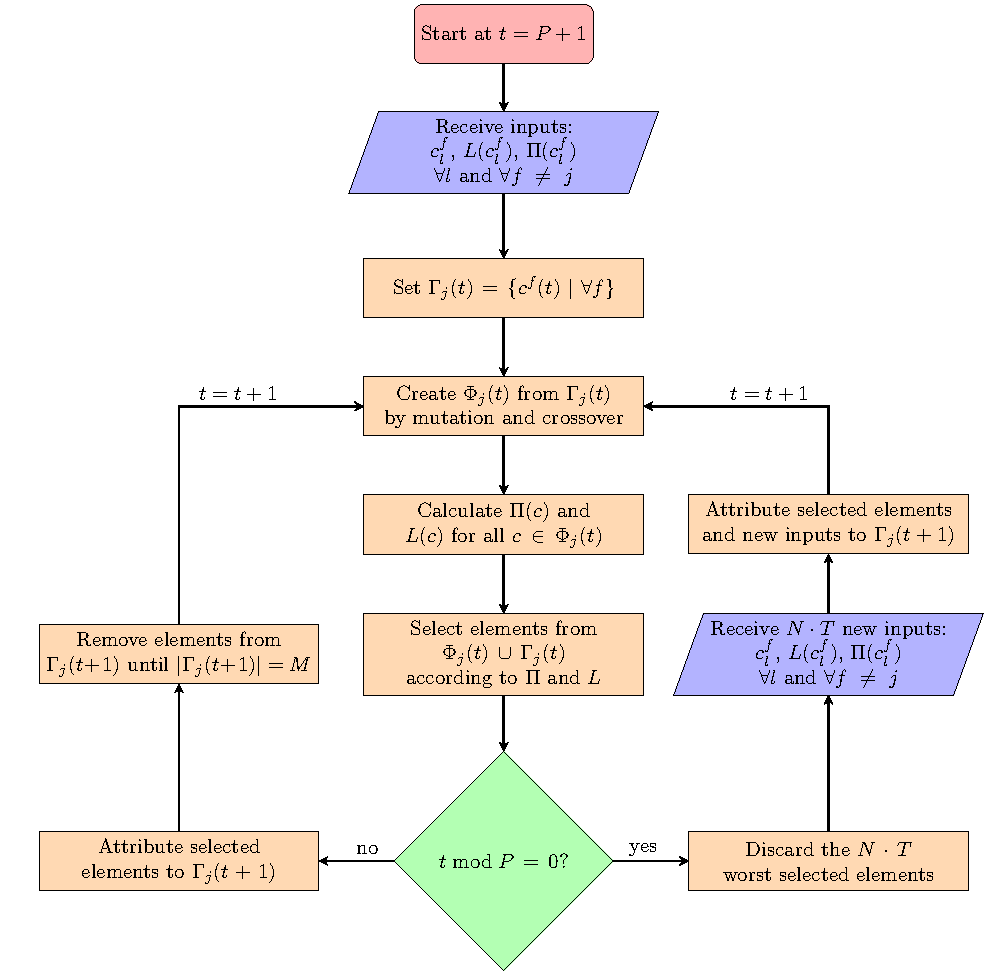
\includegraphics{AG.pdf}
\caption{Flowchart of the genetic algorithm agents use to adapt their
behaviour.}
\end{figure}

\newpage

\section{5. Results}\label{results}

To be completed

\section{6. Conclusion}\label{conclusion}

To be completed




\newpage
\singlespacing 
\bibliography{biblio.bib}

\end{document}
